\onecolumn
\appendix

\iftoggle{arxivformat} {
  % nothing
}{
  \renewcommand{\appendixpagename}{Supplementary Material}
}

\appendixpage

You can find this paper, as well as all the code necessary to run the
described experiments, in our Github repo,
\href{https://github.com/rgiordan/LinearResponseVariationalBayesNIPS2015}
{\texttt{rgiordan/LinearResponseVariationalBayesNIPS2015}}.


%========================
\section{LRVB estimates of the covariance of functions}
\label{app:function_covariance}
%========================

In \mysec{lr_subsection}, we derived an estimate of the covariance of the
natural sufficient statistics, $\theta$, of our variational approximation,
$q(\theta)$. In this section we derive a version of \eq{spec_lrvb} for the
covariance of functions of $\theta$.

We begin by estimating the covariance between $\theta$ and a function
$\phi(\theta)$. Suppose we have an MFVB solution, $q(\theta)$, to \eq{kl}.
Define the expectation of $\phi(\theta)$ to be $\mbeq\left[\phi(\theta)\right] :=
f(m)$.  This expectation is function of $m$ alone since $m$ completely
parameterizes $q$. As in \eq{perturbed_dens}, we can consider a perturbed log
likelihood that also includes $f\left(m\right)$:
%
\begin{eqnarray*}
  \log p_{t}\left(\theta\vert x \right) & = &
    \log p+t_{0}^{T}m+t_{f}f\left(m\right):=\log p+t^{T}m_{f}\\
  t & := & \left(\begin{array}{c}
  t_{0}\\
  t_{f}
  \end{array}\right) \quad \quad
  m_{f} := \left(\begin{array}{c}
  m\\
  f\left(m\right)
  \end{array}\right)
\end{eqnarray*}
%
Using the same reasoning that led to \eq{lrvb_derivative_defn}, we will define
%
$$
\truecov_{\theta \phi} = \cov_p(\theta, \phi(\theta))
  \approx \frac{dm_t^{*}}{dt_f} =: \lrcov_{\theta\phi}
$$
%
We then have the following lemma:
%
\begin{lemma} \label{lem:theta_function_covariance}
  If $\mbeq\left[\phi(\theta)\right] =: f(m)$ is a differentiable function of $m$
  with gradient $\nabla f$, then
  %
  $$
  \lrcov_{\theta\phi} = \lrcov \nabla f
  $$
  %
\end{lemma}

\begin{proof}
  %
  The derivative of the perturbed ELBO, $E_t$, is given by:
  %
  \begin{eqnarray*}
  E_{t} & := & E+t^{T}m_{f}\\
  \frac{\partial E_{t}}{\partial m} & = &
  \frac{\partial E}{\partial m}+\left(\begin{array}{cc}
  I & \nabla f\end{array}\right)\left(\begin{array}{c}
  t_{0}\\
  t_{f}
  \end{array}\right)\\
  \end{eqnarray*}
  %
  The fixed point \eq{fixed_pt} then gives:
  %
  \begin{eqnarray*}
  M_{t}\left(m\right) & := & M\left(m\right)+\left(\begin{array}{cc}
  I & \nabla f\end{array}\right)\left(\begin{array}{c}
  t_{0}\\
  t_{f}
  \end{array}\right)\\
  \frac{dm_{t}^{*}}{dt^{T}} & = &
    \left.\frac{\partial M_{t}}{\partial m^{T}}\right|_{_{m=m_{t}^{*}}}
    \frac{dm_{t}^{*}}{dt^{T}}+\frac{\partial M_{t}}{\partial t^{T}}\\
   & = & \left(\left.\frac{\partial M}{\partial m^{T}}\right|_{_{m=m_{t}^{*}}}+
   \frac{\partial}{\partial m^{T}}\left(\begin{array}{cc}
  I & \nabla f\end{array}\right)\left(\begin{array}{c}
  t_{0}\\
  t_{f}
  \end{array}\right)\right)\frac{dm^{*}}{dt^{T}}+\left(\begin{array}{cc}
  I & \nabla f\end{array}\right)
  \end{eqnarray*}
  %
  The term $\frac{\partial}{\partial m^{T}}\left(\begin{array}{cc}
  I & \nabla f\end{array}\right)\left(\begin{array}{c}
  t_{0}\\
  t_{f}
  \end{array}\right)$ is awkward, but it disappears when we evaluate at $t=0$,
  giving
  %
  \begin{eqnarray*}
  \frac{dm_{t}^{*}}{dt^{T}} & = &
    \left(\left.\frac{\partial M}{\partial m^{T}}\right|_{_{m=m_{t}^{*}}}\right)
    \frac{dm^{*}}{dt^{T}}+\left(\begin{array}{cc}
  I & \nabla f\end{array}\right)\\
   & = & \left(\frac{\partial^{2}E}{\partial m\partial m^{T}}+
    I\right)\frac{dm^{*}}{dt^{T}}+\left(\begin{array}{cc}
  I & \nabla f\end{array}\right) \Rightarrow \\
  \frac{dm^{*}}{dt^{T}} & = &
    -\left(\frac{\partial^{2}E}{\partial m\partial m^{T}}\right)^{-1}
    \left(\begin{array}{cc}I & \nabla f\end{array}\right)
  \end{eqnarray*}
  %
  Recalling that
  %
  \begin{eqnarray*}
  \frac{dm^{*}}{dt_{0}^{T}} & := & \lrcov
  \end{eqnarray*}
  %
  We can plug in to see that
  %
  \begin{equation}
  \lrcov_{\theta\phi} = \frac{dm^{*}}{dt_{f}} = \lrcov \nabla f
  \end{equation}
  %
\end{proof}
%
Finally, suppose we are interested in estimating $\cov_p(\gamma(\theta),
\phi(\theta))$, where $g(m) := \mbeq\left[\gamma(\theta)\right]$.  Again using
the same reasoning that led to \eq{lrvb_derivative_defn}, we will define
%
\begin{equation*}
\truecov_{\gamma\phi} = \cov_p(\gamma(\theta), \phi(\theta))
\approx \frac{d \mbeq\left[\gamma(\theta)\right]}{dt_f} =: \lrcov_{\gamma\phi}
\end{equation*}
%
\begin{proposition} \label{prop:function_function_covariance}
  If $\mbeq\left[\phi(\theta)\right] = f(m)$ and
  $\mbeq\left[\gamma(\theta)\right] = g(m)$ are differentiable functions of $m$
  with gradients $\nabla f$ and $\nabla g$ respectively, then
  %
  $$
    \lrcov_{\gamma\phi} = \nabla g^{T}\lrcov \nabla f
  $$
\end{proposition}
%
\begin{proof}
  By \lem{theta_function_covariance} an application of the chain rule,
  %
  \begin{eqnarray*}
  \lrcov_{\gamma\phi} =
  \frac{d \mbeq\left[\gamma(\theta)\right]}{dt_f} =
  \frac{d g\left(m\right)}{dt_f} & = & \frac{dg(m)}{dm^{T}}\frac{dm}{dt_{f}}
    =  \nabla g^{T}\lrcov \nabla f
  \end{eqnarray*}
\end{proof}

%========================
% \section{Constraints among natural parameteres or sufficient statistics}
% \label{app:constraints}
%========================

%========================
\section{Exactness of LRVB for multivariate normal means} \label{app:mvn_exact}
%========================

For any target distribution $p(\theta | x)$, it is well-known that MFVB cannot
be used to estimate the covariances between the components of $\theta$. In
particular, if $q^*$ is the estimate of $p(\theta | x)$ returned by MFVB, $q^*$
will have a block-diagonal covariance matrix---no matter the form of the
covariance of $p(\theta | x)$.

Consider approximating a multivariate Gaussian posterior distribution
$p(\theta|x)$ with MFVB. The Gaussian is the unique distribution that is fully
determined by its mean and covariance. This posterior arises, for instance,
given a multivariate normal likelihood $p(x | \mu) = \prod_{n=1:N} \gauss(x_n |
\mu, S)$ with fixed covariance $S$ and an improper uniform prior on the mean
parameter $\mu$. We make the mean field factorization assumption
$q(\mu)=\prod_{d=1:D} q(\mu_d)$, where $D$ is the total dimension of $\mu$. This
fact is often used to illustrate the shortcomings of MFVB
\cite{wang:2005:inadequacy,bishop:2006:pattern,turner:2011:two}.
In this case, it is well known that the MFVB posterior means are correct, but the
marginal variances are underestimated if $S$ is not diagonal.
However, since the posterior means are correctly estimated,
the LRVB approximation in \eq{spec_lrvb} is in fact an equality.
That is, for this model,
$\lrcov = d \mpq_t / d t^T = \truecov$ exactly.

In order to prove this result, we will rely on the following lemma.
%
\begin{lemma} \label{lem:lrvb_mvn}
%
  Consider a target posterior distribution characterized by $p(\theta | x) =
  \gauss(\theta | \mu, \Sigma)$, where $\mu$ and $\Sigma$ may depend on $x$, and
  $\Sigma$ is invertible. Let $\theta = (\theta_{1}, \ldots, \theta_{J})$, and
  consider a MFVB approximation to $p(\theta| x)$ that factorizes as $q(\theta) =
  \prod_{j} q(\theta_j)$. Then the variational posterior means are the true
  posterior means; i.e. $m_j = \mu_j$ for all $j$ between $1$ and $J$.
%
\end{lemma}

\begin{proof}
  %
  The derivation of MFVB for the multivariate normal can be found in Section
  10.1.2 of \cite{bishop:2006:pattern}; we highlight some key results here. Let
  $\Lambda = \Sigma^{-1}$. Let the $j$ index on a row or column correspond to
  $\theta_j$, and let the $-j$ index correspond to $\{\theta_{i}: i \in
  [J]\setminus j\}$. E.g., for $j=1$,
  %
  $$
    \Lambda
      = \left[ \begin{array}{ll}
          \Lambda_{11} & \Lambda_{1,-1} \\
          \Lambda_{-1,1} & \Lambda_{-1,-1}
        \end{array} \right].
  $$
  By the assumption that $p(\theta | x) = \gauss(\theta | \mu, \Sigma)$, we have
\begin{eqnarray}\label{eq:mvn_variational_dist}
  \lefteqn{\log p(\theta_{j} | \theta_{i \in [J]\setminus j}, x)} \nonumber\\
      &=& -\frac{1}{2} (\theta_{j} - \mu_{j})^{T} \Lambda_{jj} (\theta_j - \mu_j) +
         (\theta_{j} - \mu_{j})^{T} \Lambda_{j,-j} (\theta_{-j} - \mu_{-j}) + \constant,
\end{eqnarray}
%
  where the final term is constant with respect to $\theta_{j}$.
  It follows that
  \begin{align*}
    \log q^{*}_{j}(\theta_j)
      &= \mbe_{q^{*}_{i}: i \in [J]\setminus j} \log p(\theta, x) + \constant \\
      &= -\frac{1}{2} \theta_{j}^{T} \Lambda_{jj} \theta_j + \theta_j \mu_j \Lambda_{jj} - \theta_j \Lambda_{j,-j} (\mbe_{q^{*}} \theta_{-j} - \mu_{-j}).
  \end{align*}
  So
  \begin{equation*}
    q^*_j(\theta_j) = \gauss(\theta_j | m_{j}, \Lambda_{jj}^{-1}),
  \end{equation*}
  with mean parameters
  \begin{equation} \label{eq:mvn_stable_point}
    m_{j} = \mbe_{q^{*}_j} \theta_j = \mu_{j} - \Lambda_{jj}^{-1} \Lambda_{j,-j} (m_{-j} - \mu_{-j})
  \end{equation}
  as well as an equation for $\mbe_{q^{*}} \theta^T \theta$.

Note that $\Lambda_{jj}$ must be invertible, for if it were not, $\Sigma$ would
not be invertible.

The solution $m = \mu$ is a unique stable point for \eq{mvn_stable_point}, since
the fixed point equations for each $j$ can be stacked and rearranged to give
%
\begin{eqnarray*}
m-\mu & = & -\left[\begin{array}{ccccc}
0 & \Lambda_{11}^{-1}\Lambda_{12} & \cdots & \Lambda_{11}^{-1}\Lambda_{1\left(J-1\right)} & \Lambda_{11}^{-1}\Lambda_{1J}\\
\vdots &  & \ddots &  & \vdots\\
\Lambda_{JJ}^{-1}\Lambda_{J1} & \Lambda_{JJ}^{-1}\Lambda_{J2} & \cdots & \Lambda_{JJ}^{-1}\Lambda_{J\left(J-1\right)} & 0
\end{array}\right]\left(m-\mu\right)\\
 & = & -\left[\begin{array}{ccccc}
\Lambda_{11}^{-1} & \cdots & 0 & \cdots & 0\\
\vdots & \ddots &  &  & \vdots\\
0 &  & \ddots &  & 0\\
\vdots &  &  & \ddots & \vdots\\
0 & \cdots & 0 & \cdots & \Lambda_{JJ}^{-1}
\end{array}\right]\left[\begin{array}{ccccc}
0 & \Lambda_{12} & \cdots & \Lambda_{1\left(J-1\right)} & \Lambda_{1J}\\
\vdots &  & \ddots &  & \vdots\\
\Lambda_{J1} & \Lambda_{J2} & \cdots & \Lambda_{J\left(J-1\right)} & 0
\end{array}\right]\left(m-\mu\right)\Leftrightarrow\\
0 & = & \left[\begin{array}{ccccc}
\Lambda_{11} & \cdots & 0 & \cdots & 0\\
\vdots & \ddots &  &  & \vdots\\
0 &  & \ddots &  & 0\\
\vdots &  &  & \ddots & \vdots\\
0 & \cdots & 0 & \cdots & \Lambda_{JJ}
\end{array}\right]\left(m-\mu\right) +\\
&& \left[\begin{array}{ccccc}
0 & \Lambda_{12} & \cdots & \Lambda_{1\left(J-1\right)} & \Lambda_{1J}\\
\vdots &  & \ddots &  & \vdots\\
\Lambda_{J1} & \Lambda_{J2} & \cdots & \Lambda_{J\left(J-1\right)} & 0
\end{array}\right]\left(m-\mu\right)\Leftrightarrow\\
0 & = & \Lambda \left(m-\mu\right) \Leftrightarrow\\
m & = & \mu.
\end{eqnarray*}
%
The last step follows from the assumption that $\Sigma$ (and hence $\Lambda$)
is invertible.  It follows that $\mu$ is the unique stable point of
\eq{mvn_stable_point}.

\end{proof}


%%%
\begin{proposition} \label{prop:lrvb_mvn}
  Assume we are in the setting of \lem{lrvb_mvn}, where additionally
  $\mu$ and $\Sigma$ are on the interior of the feasible parameter space.
  Then the LRVB covariance estimate exactly captures the true covariance,
  $\hat{\Sigma} = \Sigma$.

\end{proposition}
%%%

\begin{proof}

  Consider the perturbation for LRVB defined in \eq{perturbed_dens}.
  By perturbing the log likelihood, we change both the true means $\mu_t$
  and the variational solutions, $m_t$. The result is a valid
  density function since the original $\mu$ and $\Sigma$ are on the
  interior of the parameter space.
  By \lem{lrvb_mvn}, the MFVB solutions are exactly the true
  means, so $m_{t,j} = \mu_{t,j}$, and the derivatives are the same
  as well.  This means that the first term in \eq{spec_lrvb} is
  not approximate, i.e.
%
  \begin{equation*}
  \frac{d \mpq_{t}}{d t^{T}}
    = \frac{d}{d t^{T}} \mbe_{p_{t}} \theta
    = \truecov_{t},
  \end{equation*}
%
  It follows from the arguments above that the LRVB covariance
  matrix is exact, and $\hat{\Sigma} = \Sigma$.

\end{proof}


%%%%%%%%%%%%%%%%%%%
\section{Comparison with supplemented expectation-maximization}\label{app:SEM}

The result in \app{mvn_exact} about the multivariate normal distribution
draws a connection between LRVB
corrections and the ``supplemented expectation-maximization'' (SEM)
method of \cite{meng:1991:using}.  SEM is an asymptotically
exact covariance correction for the EM algorithm that transforms
the full-data Fisher information matrix into the observed-data Fisher
information matrix using a correction that is formally similar to
\eq{spec_lrvb}.  In this section, we argue that this similarity
is not a coincidence; in fact the SEM correction is an
asymptotic version of LRVB with two variational blocks,
one for the missing data and one for the unknown parameters.

Although LRVB as described here requires a prior
(unlike SEM, which supplements the MLE),
the two covariance corrections coincide when
the full information likelihood is approximately log quadratic
and proportional to the posterior, $p(\theta \vert x)$.
This might be expected to occur when we have a large number
of independent data points informing each parameter---i.e.,
when a central limit theorem applies and the priors do not
affect the posterior.
In the full information likelihood, some
terms may be viewed as missing data, whereas in the Bayesian
model the same terms may be viewed as latent parameters,
but this does not prevent us from formally comparing the two methods.

We can draw a term-by-term analogy with
the equations in \cite{meng:1991:using}. We denote variables
from the SEM paper with a superscript ``$SEM$'' to avoid confusion.
MFVB does not differentiate between missing
data and parameters to be estimated, so our $\theta$ corresponds to
$(\theta^{SEM}, Y_{mis}^{SEM})$ in \cite{meng:1991:using}.
SEM is an asymptotic
theory, so we may assume that $(\theta^{SEM}, Y_{mis}^{SEM})$ have a
multivariate normal
distribution, and that we are interested in the mean and covariance of
$\theta^{SEM}$.

In the E-step of \cite{meng:1991:using}, we replace $Y_{mis}^{SEM}$ with
its conditional expectation given the data and other $\theta^{SEM}$.
This corresponds precisely to \eq{mvn_stable_point}, taking
$\theta_j = Y_{mis}^{SEM}$.  In the M-step, we find the maximum
of the log likelihood with respect to $\theta^{SEM}$, keeping
$Y_{mis}^{SEM}$ fixed at its expectation.  Since the mode
of a multivariate normal distribution is also its mean,
this, too, corresponds to \eq{mvn_stable_point}, now taking
$\theta_j = \theta^{SEM}$.

It follows that the MFVB and EM fixed point equations are the same;
i.e., our $M$ is the same as their $M^{SEM}$, and
our $\partial M / \partial m$ of \eq{dM_dt} corresponds
to the transpose of their $DM^{SEM}$, defined in \eqw{2.2.1}
of \cite{meng:1991:using}.  Since the ``complete information'' corresponds to
the variance of $\theta^{SEM}$ with fixed values for $Y_{OBS}^{SEM}$,
this is the same as our $\Sigma_{q^*,11}$, the variational covariance,
whose inverse is $I_{oc}^{-1}$.  Taken all together, this means that
equation (2.4.6) of \cite{meng:1991:using} can be
re-written as our \eq{spec_lrvb}.
%
\begin{align*}
V^{SEM} =& I_{oc}^{-1} \left(I - DM^{SEM}\right)^{-1} \Rightarrow\\
\Sigma =& \vbcov \left(I - \left(\frac{\partial M}{\partial m^T}\right)^T \right)^{-1}
       = \left(I - \frac{\partial M}{\partial m^T} \right)^{-1} \vbcov
\end{align*}

%======================
\section{Normal-Poisson details} \label{app:np_details}
%======================

In this section, we use this model to provide a detailed, step-by-step description of
a simple LRVB analysis.

The full joint distribution for the model in \eq{pn_model} is
%
\begin{align*}
\log p\left(y,z,\beta,\tau\right) &= \sum_{n=1}^{N}\left(-\frac{1}{2}\tau z_{n}^{2}+x_{n}\tau\beta z_{n}-\frac{1}{2}x_{n}^{2}\tau\beta^{2}-\frac{1}{2}\log\tau\right)\\
 &+\sum_{n=1}^{N}\left(-\exp\left(z_{n}\right)+z_{n}y_{n}\right)
 -\frac{1}{2\sigma_{\beta}^{2}}\beta^{2}+\left(\alpha_{\tau}-1\right)\log\tau-\beta_{\tau}\tau+\constant
\end{align*}
%
We find a mean-field approximation under the factorization
$q\left(\beta,\tau,z\right) =
q\left(\beta\right)q\left(\tau\right)\prod_{n=1}^{N}q\left(z_{n}\right)$. By
inspection, the log joint is quadratic in $\beta$, so the optimal
$q\left(\beta\right)$ will be Gaussian \cite{bishop:2006:pattern}. Similarly, the
log joint is a function of $\tau$ only via $\tau$ and $\log\tau$, so the optimal
$q\left(\tau\right)$ will be gamma. However, the joint does not take a standard
exponential family form in $z_n$:
%
$$
  \log p\left(z_{n}\vert y,\beta,\tau\right) = \left(x_{n}\tau\beta+y_{n}\right)z_{n}-\frac{1}{2}\tau z_{n}^{2}-\exp\left(z_{n}\right)+\constant
$$
%
The difficulty is with the term $\exp\left(z_{n}\right)$. So we make the further
restriction that
%
$$
  q\left(z_{n}\right) = \gauss\left(\cdot\right)=q\left(z_{n};\mbe\left[z_{n}\right],\mbe\left[z_{n}^{2}\right]\right).
$$
%
Fortunately, the troublesome term has an analytic expectation, as
a function of the mean parameters, under this variational posterior:
%
$$
  \mbeq\left[\exp\left(z_{n}\right)\right] = \exp\left(\mbeq\left[z_{n}\right]+\frac{1}{2}\left(\mbeq\left[z_{n}^{2}\right]-\mbeq\left[z_{n}\right]^{2}\right)\right).
$$
%
We can now write the variational distribution in terms of the following
mean parameters:
%
$$
  m = \left(\mbeq\left[\beta\right],\mbeq\left[\beta^{2}\right],\mbeq\left[\tau\right],\mbeq\left[\log\tau\right],\mbeq\left[z_{1}\right],\mbeq\left[z_{1}^{2}\right],...,\mbeq\left[z_{N}\right],\mbeq\left[z_{N}^{2}\right]\right)^{T}.
$$
%
Calculating the LRVB covariance consists of roughly four steps:

\begin{enumerate}
\item finding the MFVB optimum $q^{*}$,
\item computing the covariance $\vbcov$ of $q^*$,
\item computing $H$, the Hessian of $L(m)$, for $q^*$, and
\item computing the matrix inverse and solving $\left(I-VH\right)^{-1}V$.
\end{enumerate}

For step (1), the LRVB correction is agnostic as to how the optimum
is found. In our experiments below, we
follow a standard
coordinate ascent procedure for MFVB \cite{bishop:2006:pattern}. We analytically update
$q\left(\beta\right)$ and $q\left(\tau\right)$.
Given $q\left(\beta\right)$ and $q\left(\tau\right)$, finding the
optimal $q\left(z\right)$ becomes $N$ separate two-dimensional optimization
problems; there is one dimension for each of the mean parameters $\mbeq \left[ z_n \right]$ and $\mbeq \left[ z_n^2 \right]$.
In our examples, we solved these problems sequentially using
IPOPT \cite{ipopt:package}.

To compute $\vbcov$ for step (2),
we note that by the mean-field assumption,
$\beta$, $\tau$, and $z_{n}$ are independent, so $\vbcov$ is block
diagonal. Since we have chosen convenient variational distributions,
the mean parameters have known covariance matrices. For example, from
standard properties of the normal distribution,
$\textrm{Cov}\left(\beta,\beta^{2}\right)=2\mbeq\left[\beta\right]$$\left(\mbeq\left[\beta^{2}\right]-\mbeq\left[\beta\right]^{2}\right)$.

For step (3), the mean parameters for $\beta$ and $\tau$ co-occur with each other
and with all the $z_{n}$, so these four rows of $H$ are expected
to be dense. However, the mean parameters for $z_{n}$ never occur
with each other, so the bulk of $H$---the $2N\times2N$ block corresponding
to the mean parameters of $z$---will be block diagonal (\fig{H_sparse}).
The Hessian of $L\left(m\right)$ can be calculated analytically,
but we used the autodifferentiation software \texttt{JuMP} \cite{JuMP:LubinDunningIJOC}.

Finally, for step (4),
we use the technique in \mysec{scaling_formulas}
to exploit the sparsity of $\vbcov$ and $H$ (\fig{IVH_sparse}) in calculating $(I-VH)^{-1}$.

\begin{figure}[ht!]
  \centering
  \begin{subfigure}{0.3\linewidth}
    \centering
    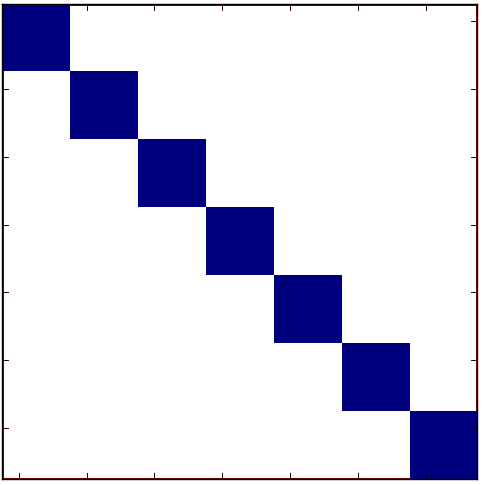
\includegraphics[height=0.3 \linewidth]{./static_images/cov_modified.png}
    \caption{\label{fig:V_sparse} MFVB covariance $V$}
  \end{subfigure}
  \begin{subfigure}{0.3\linewidth}
    \centering
    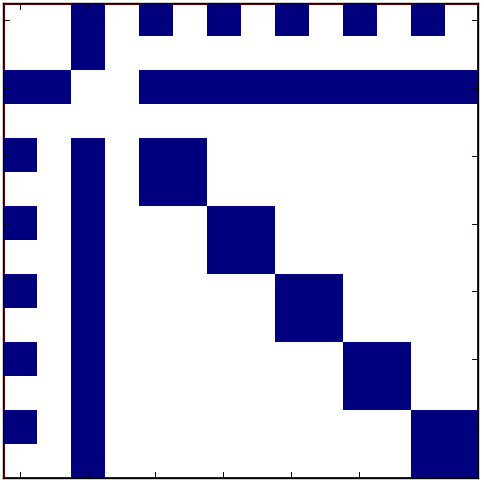
\includegraphics[height=0.3 \linewidth]{./static_images/hessian_modified.png}
    \caption{\label{fig:H_sparse} Hessian matrix $H$}
  \end{subfigure}
  \begin{subfigure}{0.3\linewidth}
    \centering
    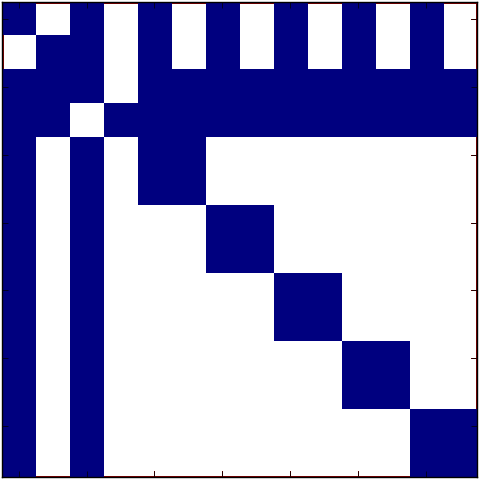
\includegraphics[height=0.3 \linewidth]{./static_images/lrvb_modified.png}
    \caption{\label{fig:IVH_sparse} \mbox{$(I - VH)$}}
  \end{subfigure}
  \caption{Sparsity patterns for $\hat\truecov = (I - VH)^{-1}$ using the model in \eq{pn_model}, $n = 5$ (white = 0)}
  \label{fig:sparsity_patterns}
\end{figure}



%======================
\section{Random effects model details} \label{app:re_details}
%======================

As introduced in \mysec{random_effects_model}, our model is:
%
\begin{eqnarray*}
y_{n}\vert\beta,z,\tau & \indep & \gauss\left(\beta^{T}x_{n}+r_{n}z_{k\left(n\right)},\tau^{-1}\right)\\
z_{k}\vert\nu & \iid & \gauss\left(0,\nu^{-1}\right)
\end{eqnarray*}
%
With the priors:
%
\begin{eqnarray*}
\beta & \sim & \gauss\left(0,\Sigma_{\beta}\right)\\
\nu & \sim & \Gamma\left(\alpha_{\nu},\beta_{\nu}\right)\\
\tau & \sim & \Gamma\left(\alpha_{\tau},\beta_{\tau}\right)
\end{eqnarray*}
%
We will make the following mean field assumption:
%
\begin{eqnarray*}
q\left(\beta,z,\tau,\nu\right) & = & q\left(\nu\right)q\left(\tau\right)q\left(\beta\right)\prod_{k=1}^{K}q\left(z_{k}\right)
\end{eqnarray*}
%
We have $n\in\left\{ 1,...,N\right\} $, and $k\in\left\{ 1,...,K\right\} $,
and $k\left(n\right)$ matches an observation $n$ to a random effect
$k$, allowing repeated observations of a random effect. The full
joint log likelihood is:
%
\begin{eqnarray*}
\log p\left(y_{n}\vert z_{k\left(n\right)},\tau,\beta\right) & = & -\frac{\tau}{2}\left(y_{n}-\beta^{T}x_{n}-r_{n}z_{k\left(n\right)}\right)^{2}+\frac{1}{2}\log\tau+\constant\\
\log p\left(z_{k}\vert\nu\right) & = & -\frac{\nu}{2}z_{k}^{2}+\frac{1}{2}\log\nu+\constant\\
\log p\left(\beta\right) &  & -\frac{1}{2}\textrm{trace}\left(\Sigma_{\beta}^{-1}\beta\beta^{T}\right)+\constant\\
\log p\left(\tau\right) & = & \left(\alpha_{\tau}-1\right)\log\tau-\beta_{\tau}\tau+\constant\\
\log p\left(\nu\right) & = & \left(\alpha_{\nu}-1\right)\log\nu-\beta_{\nu}\nu+\constant\\
\log p\left(y,\tau,\beta,z\right) & = & \sum_{n=1}^{N}\log p\left(y_{n}\vert z_{k\left(n\right)},\tau,\beta\right)+\sum_{k=1}^{K}\log p\left(z_{k}\vert\nu\right)+\\
 &  & \log p\left(\beta\right)+\log p\left(\nu\right)+\log p\left(\tau\right)
\end{eqnarray*}
%
Expanding the first term of the conditional likelihood of $y_{n}$
gives
%
\begin{eqnarray*}
\lefteqn{-\frac{\tau}{2}\left(y_{n}-\beta^{T}x_{n}-r_{n}z_{k\left(n\right)}\right)^{2}}\\
& = & -\frac{\tau}{2}\left(y_{n}^{2}-2y_{n}x_{n}^{T}\beta-2y_{n}r_{n}z_{n\left(k\right)}+\textrm{trace}\left(x_{n}x_{n}^{T}\beta\beta^{T}\right)+r_{n}^{2}z_{k\left(n\right)}^{2}+2r_{n}x_{n}^{T}\beta z_{k\left(n\right)}\right)
\end{eqnarray*}
%
By grouping terms, we can see that the mean parameters will be
%
\begin{eqnarray*}
q\left(\beta\right) & = & q\left(\beta;\mbeq\left[\beta\right],\mbeq\left[\beta\beta^{T}\right]\right)\\
q\left(z_{k}\right) & = & q\left(z_{k};\mbeq\left[z_{k}\right],\mbeq\left[z_{k}^{2}\right]\right)\\
q\left(\tau\right) & = & q\left(\tau;\mbeq\left[\tau\right],\mbeq\left[\log\tau\right]\right)\\
q\left(\nu\right) & = & q\left(\nu;\mbeq\left[\nu\right],\mbeq\left[\log\nu\right]\right)
\end{eqnarray*}
%
It follows that the optimal variational distributions are $q\left(\beta\right)=$multivariate
normal, $q\left(z_{k}\right)=$univariate normal, and $q\left(\tau\right)$
and $q\left(\nu\right)$ will be gamma. We performed standard coordinate
ascent on these distributions \cite{bishop:2006:pattern}.

As in \mysec{normal_poisson_model}, we implemented this model in the
autodifferentiation software JuMP \cite{JuMP:LubinDunningIJOC}.
This means conjugate coordinate updates were easy, since the natural
parameters corresponding to a mean parameters are the first derivatives
of the log likelihood with respect to the mean parameters. For example,
denoting the log likelihood at step $s$ by $L_{s}$, the update for
$q_{s+1}\left(z_{k}\right)$ will be:
%
\begin{eqnarray*}
\log q_{s+1}\left(z_{k}\right) & = & \frac{\partial\mbeq\left[L_{s}\right]}{\partial\mbeq\left[z_{k}\right]}z_{k}+\frac{\partial\mbeq\left[L_{s}\right]}{\partial\mbeq\left[z_{k}^{2}\right]}z_{k}^{2}+\constant
\end{eqnarray*}
%
Given the partial derivatives of $L_{s}$ with respect to the mean
parameters, the updated mean parameters for $z_{k}$ can be read off
directly using standard properties of the normal distribution.

The variational covariance matrices are all standard. We can see that
$H$ will have nonzero terms in general (for example, the three-way
interaction $\mbeq\left[\tau\right]\mbeq\left[z_{k\left(n\right)}\right]\mbeq\left[\beta\right]$),
and that LRVB will be different from MFVB. As usual in our models,
$H$ is sparse, and we can easily apply the technique in section \mysec{scaling_formulas}
to get the covariance matrix excluding the random effects, $z$.

%======================
\section{Multivariate normal mixture details} \label{app:mvn_details}
%======================

In this section we derive the basic formulas needed to calculate \eq{spec_lrvb}
for a finite mixture of normals, which
is the model used in \mysec{experiments}.  We will
follow the notation introduced in \mysec{normal_mixture_model}.

Let each observation, $x_{n}$, be a $P\times1$ vector. We will denote
the $P$th component of the $n$th observation $x_{n}$, with a
similar pattern for $z$ and $\mu$. We will denote the $p$, $q$th
entry in the matrix $\Lambda_{k}$ as $\Lambda_{k,pq}$. The data
generating process is as follows:
%
\begin{eqnarray*}
P\left(x | \mu, \pi, \Lambda \right) &=&
  \prod_{n=1}^N P\left(x_{n}|z_{n},\mu,\Lambda \right)
  \prod_{k=1}^{K} P\left(z_{nk}|\pi_{k} \right)\\
\log P\left(x_{n}|z_{n},\mu,\Lambda\right) & = &
    \sum_{n=1}^{N}z_{nk}\log\phi_{k}(x_{n}) + \constant\\
\log\phi_{k}(x) & = & -\frac{1}{2}\left(x - \mu_{k}\right)^{T} \Lambda_{k}\left(x-\mu_{k}\right) +
    \frac{1}{2}\log\left|\Lambda_{k}\right|+ \constant\\
\log P(z_{nk}|\pi_{k}) & = & \sum_{k=1}^{K}z_{nk}\log\pi_{k} + \constant
\end{eqnarray*}
%
It follows that the log posterior is given by
%
\begin{eqnarray*}
\log P(z,\mu,\pi,\Lambda | x) & = & \sum_{n=1}^{N}\sum_{k=1}^{K}z_{nk}\left(\log\pi_{k}-\frac{1}{2}\left(x_{n}-\mu_{k}\right)^{T}\Lambda_{k}\left(x_{n}-\mu_{k}\right)+\frac{1}{2}\log\left|\Lambda_{k}\right|\right) + \\
  &  & \sum_{k=1}^{K} \log p(\mu_{k}) + \sum_{k=1}^{K} \log p(\Lambda_{k}) +
        \log p(\pi) + \constant
\end{eqnarray*}
%
We used a multivariate normal prior for $\mu_{k}$, a Wishart prior for
$\Lambda_{k}$, and a Dirichlet prior for $\pi$.  In the simulations described
in \mysec{normal_mixture_model}, we used the following prior parameters
for the VB model:
%
\begin{eqnarray*}
  p(\mu_{k}) &=& \mathcal{N}\left(0_P, \textrm{diag}_P(0.01)^{-1}\right) \\
  p(\Lambda_{k}) &=& \textrm{Wishart}(\textrm{diag}_P(0.01), 1)\\
  p(\pi) &=& \textrm{Dirichlet}(5_K)
\end{eqnarray*}
%
Here, $\textrm{diag}_P(a)$ is a $P$-dimensional diagonal matrix with $a$ on the
diagonal, and $0_P$ is a length $P$ vector of the value $0$, with a similar
definition for $5_K$. Unfortunately, the function we used for the MCMC
calculations, \texttt{rnmixGibbs} in the package \texttt{bayesm}, uses a
different form for the $\mu_{k}$ prior. Specifically, \texttt{rnmixGibbs} uses
the prior
%
$$
  p_{MCMC}\left(\mu_{k} \right \vert \Lambda_{k}) =
    \mathcal{N}(0, a^{-1} \Lambda_{k}^{-1})
$$
%
where $a$ is a scalar.  There is no way to exactly match
$p_{MCMC}(\mu_k)$ to $p(\mu_k)$, so we simply set $a=0.01$.
Since our datasets are all reasonably large, the prior was dominated by the
likelihood, and we found the results extremely insensitive to the prior
on $\mu_{k}$, so this discrepancy is of no practical importance.

The parameters $\mu_{k}$, $\Lambda_{k}$, $\pi$, and $z_{n}$ will
each be given their own variational distribution.  For $q_{\mu_k}$ we will
use a multivariate normal distribution; for $q_{\Lambda_{k}}$ we will
us a Wishart distirbution; for $q_{\pi}$ we will use a Dirichlet distribution;
for $q_{z_{n}}$ we will use a Multinoulli (a single multinomial draw).  These
are all the optimal variational choices given the mean field assumption and
the conditional conjugacy in the model.

The sufficient statistics for $\mu_{k}$ are all terms of the form
$\mu_{kp}$ and $\mu_{kp}\mu_{kq}$. Consequently, the sub-vector
of $\theta$ corresponding to $\mu_{k}$ is
%
\begin{eqnarray*}
\theta_{\mu_{k}} & = & \left(\begin{array}{c}
\mu_{k1}\\
\vdots\\
\mu_{kp}\\
\mu_{k1}\mu_{k1}\\
\mu_{k1}\mu_{k2}\\
\vdots\\
\mu_{kP}\mu_{kP}
\end{array}\right)
\end{eqnarray*}
%
We will only save one copy of $\mu_{kp}\mu_{kq}$ and $\mu_{kq}\mu_{kp}$,
so $\theta_{\mu_{k}}$ has length $P+\frac{1}{2}\left(P+1\right)P$.
For all the parameters, we denote the complete stacked vector without
a $k$ subscript:
%
\begin{eqnarray*}
\theta_{\mu} & = & \left(\begin{array}{c}
\theta_{\mu_{1}}\\
\vdots\\
\theta_{\mu_{K}}
\end{array}\right)
\end{eqnarray*}
%
The sufficient statistics for $\Lambda_{k}$ are all the terms $\Lambda_{k,pq}$
and the term $\log\left|\Lambda_{k}\right|$. Again, since $\Lambda$ is
symmetric, we do not keep redundant terms, so $\theta_{\Lambda_{k}}$ has length
$1+\frac{1}{2}\left(P+1\right)P$. The sufficient statistic for $\pi$ is the
$K$-vector $\left(\log\pi_{1},...,\log\pi_{K}\right)$. The sufficient statistics
for $z$ are simply the $N\times K$ values $z_{nk}$ themselves.

In terms of \mysec{scaling_formulas}, we have
%
\begin{eqnarray*}
\alpha & = & \left(\begin{array}{c}
\theta_{\mu}\\
\theta_{\Lambda}\\
\theta_{\pi}
\end{array}\right)\\
z & = & \left(\begin{array}{c}
\theta_{z}\end{array}\right)
\end{eqnarray*}
%
That is, we are primarily interested in the covariance of the sufficient
statistics of $\mu$, $\Lambda$, and $\pi$.  The latent variables $z$ are
nuisance parameters.

To put the log likelihood in terms useful for LRVB, we must express
it in terms of the sufficient statistics, taking into account the
fact the $\theta$ vector does not store redundant terms (e.g. it
will only keep $\Lambda_{ab}$ for $a<b$ since $\Lambda$ is symmetric).
%
\begin{eqnarray*}
  \lefteqn{-\frac{1}{2}\left(x_{n}-\mu_{k}\right)^{T}\Lambda_{k}\left(x_{n}-\mu_{k}\right)} \\
 & = & -\frac{1}{2}\textrm{trace}\left(\Lambda_{k}\left(x_{n}-\mu_{k}\right)\left(x_{n}-\mu_{k}\right)^{T}\right)\\
 & = & -\frac{1}{2}\sum_{a}\sum_{b}\left(\Lambda_{k,ab}\left(x_{n,a}-\mu_{k,a}\right)\left(x_{n,b}-\mu_{k,b}\right)\right)\\
 & = & -\frac{1}{2}\sum_{a}\sum_{b}\left(\Lambda_{k,ab}\mu_{k,a}\mu_{k,b}-\Lambda_{k,ab}x_{n,a}\mu_{k,b}-
          \Lambda_{k,ab}x_{n,b}\mu_{k,a}+\Lambda_{k,ab}x_{n,a}x_{n,b}\right)\\
 & = & -\frac{1}{2}\sum_{a}\Lambda_{k,aa}\left(\mu_{k}^{2}\right)^{a}+\sum_{a}\Lambda_{k,aa}x_{n,a}\mu_{k,a}-\frac{1}{2}\sum_{a}\Lambda_{k,aa}\left(x_{n}^{2}\right)^{2}-\\
 &  & \frac{1}{2}\sum_{a\ne b}\Lambda_{k,ab}\mu_{k,a}\mu_{k,b}+\sum_{a\ne b}\Lambda_{k,ab}x_{n,a}\mu_{k,b}-\frac{1}{2}\sum_{a\ne b}\Lambda_{k,ab}x_{n,a}x_{n,b}\\
 & = & -\frac{1}{2}\sum_{a}\Lambda_{k,aa}\left(\mu_{k}^{2}\right)^{a}+\sum_{a}\Lambda_{k,aa}x_{n,a}\mu_{k,a}-\frac{1}{2}\sum_{a}\Lambda_{k,aa}\left(x_{n}^{2}\right)^{2}-\\
 &  & \sum_{a<b}\Lambda_{k,ab}\mu_{k,a}\mu_{k,b}+\sum_{a<b}\Lambda_{k,ab}\left(x_{n,a}\mu_{k,b}+x_{n,b}\mu_{k,a}\right)-\sum_{a<b}\Lambda_{k,ab}x_{n,a}x_{n,b}
\end{eqnarray*}
%
The MFVB updates and covariances in $V$ are all given by properties of standard
distributions. To compute the LRVB corrections, it only remains to calculate the
Hessian, $H$. These terms can be read directly off the posterior. First we
calculate derivatives with respect to components of $\mu$.
%
\begin{eqnarray*}
\frac{\partial^{2}H}{\partial\mu_{k,a}\partial\Lambda_{k,ab}} & = & \sum_{i}z_{nk}x_{n,b}\\
\frac{\partial^{2}H}{\partial\left(\mu_{k,a}\mu_{k,b}\right)\partial\Lambda_{k,ab}} & = & -\left(\frac{1}{2}\right)^{1(a=b)}\sum_{n}z_{nk}\\
\frac{\partial^{2}H}{\partial\mu_{k,a}\partial z_{nk}} & = & \sum_{b}\Lambda_{k,ab}x_{n,b}\\
\frac{\partial^{2}H}{\partial\left(\mu_{k,a}\mu_{k,b}\right)\partial z_{nk}} & = & -\left(\frac{1}{2}\right)^{1(a=b)}\Lambda_{k,ab}
\end{eqnarray*}
%
All other $\mu$ derivatives are zero. For $\Lambda$,
%
\begin{eqnarray*}
\frac{\partial^{2}H}{\partial\Lambda_{k,ab}\partial z_{nk}} & = & -\left(\frac{1}{2}\right)^{1(a=b)}\left(x_{n,a}x_{n,b}-\mu_{k,a}x_{n,b}-\mu_{k,b}x_{n,a}+\mu_{k,a}\mu_{k,b}\right)\\
\frac{\partial^{2}H}{\partial\log\left|\Lambda_{k}\right|\partial z_{nk}} & = & \frac{1}{2}
\end{eqnarray*}
%
The remaining $\Lambda$ derivatives are zero. The only nonzero second
derivatives for $\log\pi$ are to $Z$ and are given by
%
\begin{eqnarray*}
\frac{\partial^{2}H}{\partial\log\pi_{k}\partial z_{nk}} & = & 1
\end{eqnarray*}
%
Note in particular that $H_{zz} = 0$, allowing efficient calculation of
\eq{nuisance_lrvb_est}.

%======================
\section{MNIST details} \label{app:mnist_details}
%======================

For a real-world example,
we applied LRVB to the unsupervised classification of two digits
from the MNIST dataset of handwritten digits.
We first preprocess the MNIST dataset by performing principle component
analysis on the training data's centered pixel intensities
and keeping the top $\MNISTp$ components.
For evaluation, the test data is projected onto the same
$\MNISTp$-dimensional subspace found using the training data.

We then treat the problem of
separating handwritten $0$s from $1$s as an unsupervised clustering
problem.  We limit the dataset to instances labeled as $0$
or $1$, resulting in $\MNISTn$ training and $\MNISTTestN$ test points.
We fit the training data
as a mixture of multivariate Gaussians.  Here, $K=2$, $P=\MNISTp$, and
$N=\MNISTn$.  Then, keeping the $\mu$, $\Lambda$, and $\pi$
parameters fixed, we calculate the expectations of the
latent variables $z$ in \eq{normal_mixture_model} for the test set.
We assign test set data point $x_n$ to whichever component has
maximum a posteriori expectation.  We count successful classifications
as test set points that match their cluster's majority label
and errors as test set points that are different from their cluster's
majority label.  By this measure, our test set error rate was
$\MNISTTestError$. We stress that we intend only to demonstrate
the feasibility of LRVB on a large, real-world dataset rather than
to propose practical methods for modeling MNIST.
